Assuming $\delta v = 0$, the non-linear model of the system is formulated. This non-linear model is then simulated using a square wave and a chirp input covering the entire operating range in terms of amplitude. The simulation results are compared with experimental data.

Fig.-\ref{fig::sq_valid} and Fig.-\ref{fig::chirp_valid} display the responses
to square wave and chirp inputs, respectively. These figures indicate that the
model parameters are estimated with reasonable accuracy. Any discrepancies
between the simulation and experimental data can primarily be attributed to the
real-time estimation of $\delta v$.
%===
\begin{figure}[h]
    \centering
    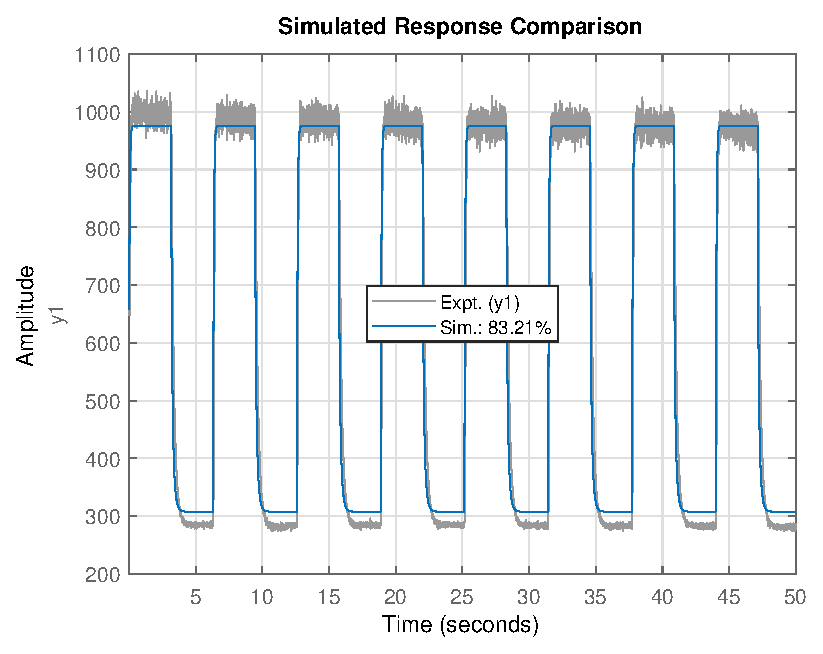
\includegraphics[width = \figsize]{./figs/nl_valid/square_validation.eps}
    \caption{Square Wave Input Response}
    \label{fig::sq_valid}
\end{figure}
\begin{figure}[h]
    \centering
    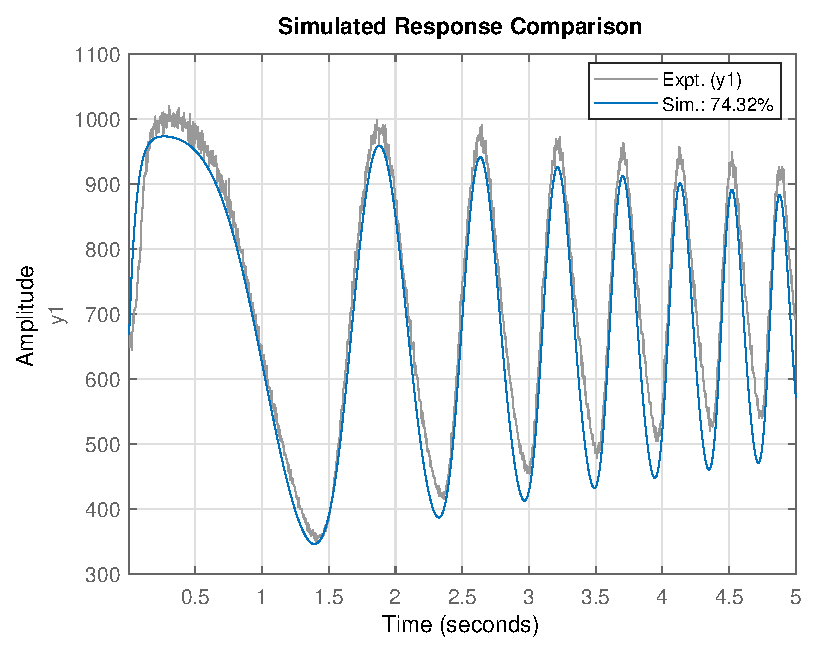
\includegraphics[width = \figsize]{./figs/nl_valid/chirp_validation.eps}
    \caption{Chirp Input Response}
    \label{fig::chirp_valid}
\end{figure}
